% ==============================================================================
% reports/tables.tex — Publication Tables in LaTeX booktabs format
% SYNTHETIC DATA -- pipeline test only
% ==============================================================================

% --- Table 1: Corpus Descriptives ---
\begin{table}[t]
\centering
\small
\caption{Corpus Characteristics Before and After Quality Filtration (\textit{SYNTHETIC DATA -- pipeline test only})}
\label{tab:corpus_descriptives}
\begin{tabular}{lrrrrr}
\toprule
\textbf{Sample Stage / Strata} & \textbf{Records ($N$)} & \textbf{Replika} & \textbf{Character.AI} & \textbf{Total Words} & \textbf{Excluded} \\
\midrule
Raw Synthetic Pool & 360 & 188 & 172 & 54,435 & --- \\
\quad Excluded: $w < 100$ words & 152 & 83 & 69 & --- & 152 \\
\quad Excluded: $w > 3,000$ words & 1 & 0 & 1 & --- & 1 \\
\quad Excluded: Sessions $\notin [1, 21]$ & 4 & 2 & 2 & --- & 4 \\
\quad Excluded: Student unknown & 56 & 28 & 28 & --- & 56 \\
\midrule
\textbf{Final Analysis Dataset} & \textbf{171} & \textbf{90} & \textbf{81} & \textbf{33,754} & \textbf{189} \\
\quad Group 1: $<1$ month & 38 & 17 & 21 & 7,593 & --- \\
\quad Group 2: $1$--$3$ months & 57 & 32 & 25 & 12,175 & --- \\
\quad Group 3: $>3$ months & 76 & 41 & 35 & 13,986 & --- \\
\bottomrule
\end{tabular}
\end{table}

% --- Table 2: RQ2 Results ---
\begin{table}[t]
\centering
\small
\caption{Emotional Dependence Marker Frequency ($F_i$) and Non-Parametric Group Comparisons (\textit{SYNTHETIC DATA -- pipeline test only})}
\label{tab:rq2_results}
\begin{tabular}{lrrrrrr}
\toprule
\textbf{Group / Metric} & \textbf{$n$} & \textbf{Median} & \textbf{IQR} & \textbf{$p_{25}$--$p_{75}$} & \textbf{Mean} & \textbf{SD} \\
\midrule
$<1$ month ($G_1$) & 38 & 10.69 & 9.58 & 6.03--15.61 & 11.03 & 7.81 \\
$1$--$3$ months ($G_2$) & 57 & 11.70 & 12.02 & 7.30--19.32 & 13.52 & 9.36 \\
$>3$ months ($G_3$) & 76 & \textbf{20.78} & 23.93 & 9.31--33.24 & 24.59 & 22.77 \\
\midrule
\multicolumn{7}{l}{\textbf{Hypothesis Tests ($H_0$: no difference vs $H_1$: monotonic increase)}} \\
\multicolumn{3}{l}{Mann--Whitney $U$ ($G_3 > G_1$)} & \multicolumn{4}{l}{$U = 2079.5$, $p = 6.73e-05$ ($p < 0.001$)} \\
\multicolumn{3}{l}{Cliff's delta ($\delta$) [95\% CI]} & \multicolumn{4}{l}{\textbf{0.440} [0.250, 0.614] (medium--large effect)} \\
\multicolumn{3}{l}{Kruskal--Wallis omnibus ($H$)} & \multicolumn{4}{l}{$H = 19.15$, $p = 6.95e-05$ ($p < 0.001$)} \\
\multicolumn{3}{l}{Jonckheere--Terpstra trend ($J$)} & \multicolumn{4}{l}{$J = 6206.5$, $Z = 4.35$, $p = 6.67e-06$ ($p < 0.001$)} \\
\bottomrule
\end{tabular}
\end{table}

% --- Table 3: RQ3 Results ---
\begin{table}[t]
\centering
\small
\caption{Association of Usage Intensity with the Isolation--Avoidance Index ($I_i$) (\textit{SYNTHETIC DATA -- pipeline test only})}
\label{tab:rq3_results}
\begin{tabular}{llrrrl}
\toprule
\textbf{Model / Specification} & \textbf{Predictor Variable} & \textbf{Estimate / $\rho_s$} & \textbf{$p$-value} & \textbf{$N$} & \textbf{Interpretation} \\
\midrule
\textbf{Bivariate Monotonic} & Duration (months) & $\rho_s = 0.136$ & $0.038$ & 171 & Statistically significant trend \\
& Sessions per week & $\rho_s = 0.082$ & $0.144$ & 171 & Null retained ($p > 0.05$) \\
\midrule
\textbf{Controlled Regression} & Intercept ($\beta_0$) & $7.897$ & --- & 171 & Baseline avoidance rate \\
($I_i \sim \text{Dur} + \text{Sess}$) & Duration ($\beta_1$) & $-0.129$ & --- & 171 & Adjusted monthly change \\
& Sessions ($\beta_2$) & $-0.619$ & --- & 171 & Adjusted session change \\
\bottomrule
\end{tabular}
\end{table}

% --- Figure Subcaption LaTeX Environment ---
\begin{figure}[t]
\centering
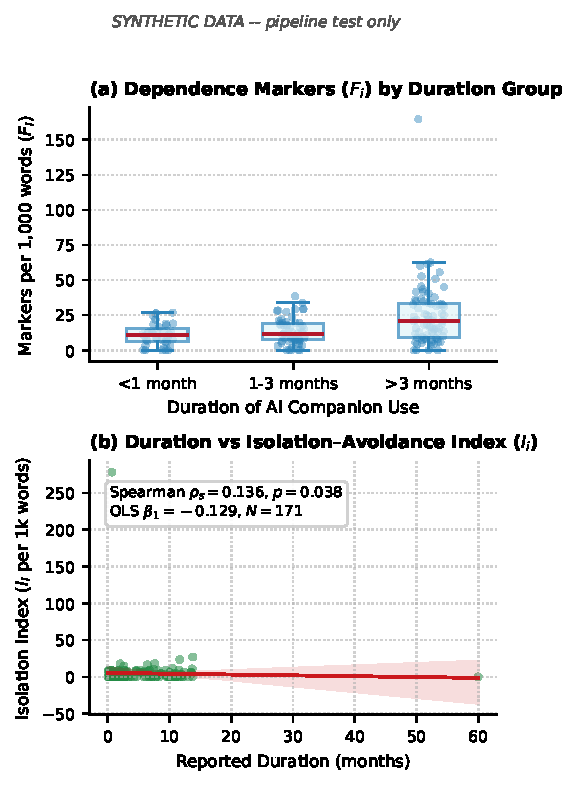
\includegraphics[width=\columnwidth]{reports/figures/study/study_results.pdf}
\caption{Quantitative findings for emotional dependence and social avoidance across duration strata (\textit{SYNTHETIC DATA -- pipeline test only}). (a) Boxplots with overlaid strip observations show dependence markers per 1,000 words ($F_i$) across three usage durations. Whiskers span $1.5 \times \text{IQR}$; central line represents the group median. (b) Bivariate relationship between interaction duration (months) and the isolation--avoidance index ($I_i$). The solid red line indicates the linear OLS fit; shaded band shows the 95\% bootstrap confidence interval ($B = 1,000$ resamples).}
\label{fig:study_results}
\end{figure}
